\documentclass{school-22.211-notes}
\date{April 30, 2012}

\begin{document}
\maketitle

\lecture{Point Kinetics With Feedbacks}
Feedback matters as demonstrated in Fig.~\ref{feedback}. 
\begin{figure}[ht]
\centering
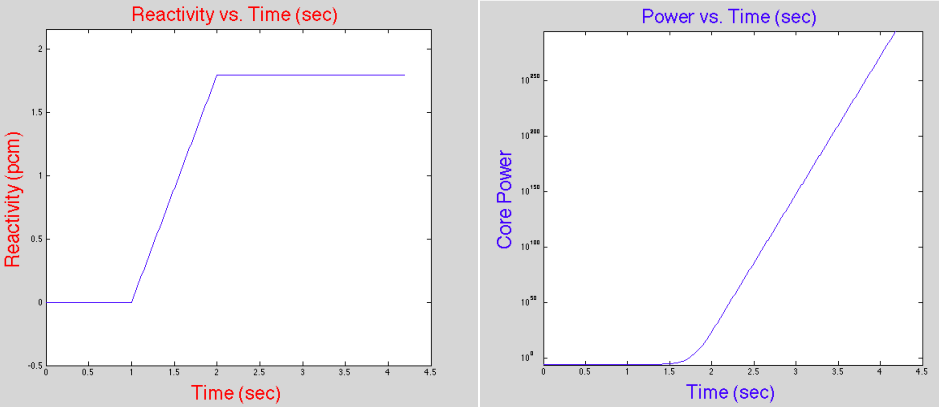
\includegraphics[width=4in]{images/pke/feedback1.png}
\\
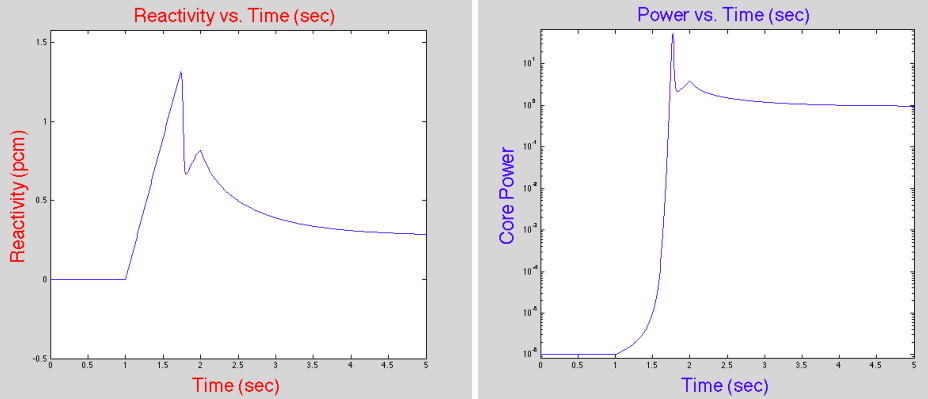
\includegraphics[width=4in]{images/pke/feedback2.png}
\caption{\$1.5 RIA With or Without Doppler Feedback}\label{feedback}
\end{figure}

\clearpage
\topic{Fuchs-Nordheim Model}
The Fuchs-Nordheim Model predicts the shape and the magnitude of the transient. We do not really solve the analytical solution of this model, but instead study some characteristics from it. 

\subtopic{Assumptions}
To start, we make three assumptions, 
\begin{enumerate}
\item If $\rho \gg \beta$, we can ignore the delayed neutrons and hence write the power distribution $P(t)$ as the 1st equation in PKE (we use $P(t)$ instead of $T(t)$ for the shape function now to avoid the confusion with temperature $T$ that we would use repeatively in this section). 
  \eqn{ \ddt P(t) &= \frac{\rho(t) - \beta}{\Lambda} P(t) + \Sum_i \lambda_i C_i (t) \approx \frac{\rho(t) - \beta}{\Lambda} P(t) \label{fn-eq1}}
  It is fair to ignore the precursors, because as in Fig.~\ref{fn1} top row, we can see that the power with precursor is small enough that the F-N model provides good approximation. The bottom row of Fig.~\ref{fn1} is plotted on a log-log scale to show the small difference made by the precursors.  
\begin{figure}[ht]
  \centering
  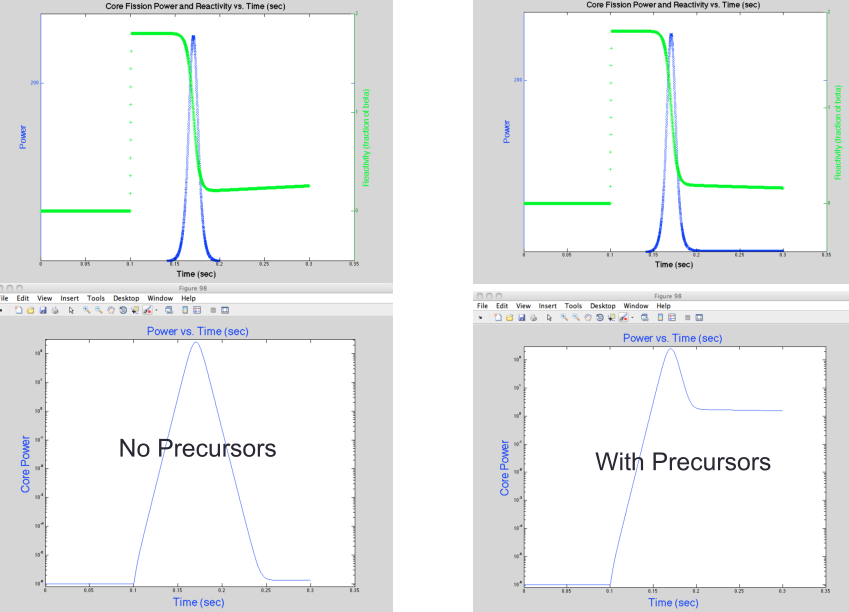
\includegraphics[width=4in]{images/pke/fn1.png}
  \caption{Assumption in Fuchs-Nordheim: No Precursors}\label{fn1}
\end{figure}

\item If transient is so rapid that no heat transferred form the fuel \footnote{The time constant for heat to be removed from \ce{UO_2} fuel is about 5 mins.}, 
  \eqn{ T_{fuel} = T_{fuel}^0 + \frac{1}{C_p} \int P(t) \dt \label{fn-eq2} }

\item Assume a Doppler Feedback coefficient independent of temperature (recall that we calculated the doppler we calculated is about 3 pcm), 
  \eqn{ \rho(t) = \rho_{rod} - \alpha (T_{fuel} - T_{fuel}^0) \label{fn-eq3} }
\end{enumerate}

\subtopic{First Derivation}
Then we solve a first order ODE. We manipulate Eq.~\ref{fn-eq2} to get,
\eqn{ \frac{\dT_{fuel} (t)}{\dt} = \frac{P(t)}{C_p} \label{fn-eq4}}
Plug Eq.~\ref{fn-eq3} into Eq.~\ref{fn-eq1} (omit $T_{fuel}^0$), 
\eqn{ \frac{\dP(t)}{\dt} = \frac{\rho_{rod} - T_{fuel} - \beta}{\Lambda} P(t) \label{fn-eq5} }
Eq.~\ref{fn-eq5} divided by \ref{fn-eq4}, 
\begin{align}
\frac{\dP(t)}{\dT_{fuel}} &= \frac{\frac{\dP(t)}{\dt}}{\frac{\dT_{fuel} (t)}{\dt}} =  \frac{(\rho_{rod} - T_{fuel} - \beta ) C_p}{\Lambda} \\
&= \frac{1}{\Lambda} \left[ C_p (\rho_{rod} - \beta) - \alpha C_p T_{fuel} (t) \right] \\
\Aboxed{ P(t) &= P_0 + \frac{1}{\Lambda} \left[ C_p (\rho_{rod} - \beta) T_{fuel} (t)  - \frac{\alpha C_p}{2} T^2_{fuel} (t) \right]  } \label{fn-power}
\end{align}
Eq.~\ref{fn-power} can be used to find peak power behavior. For peak power, we set $\frac{\dP}{dT_{fuel}} = 0$, thus, 
\begin{align}
0 &= \frac{1}{\Lambda} \left[ C_p (\rho_{rod} - \beta) - C_p \alpha T_{fuel}^{peak} \right] \\
\Aboxed{ T_{fuel}^{peak} &= \frac{\rho_{rod} - \beta}{\alpha} } \label{fn-11} \\
\Aboxed{ P^{peak} &= P_0 + \frac{C_p (\rho_{rod} - \beta)^2}{2 \Lambda \alpha} }
\end{align}
It is important to notice that peak temperature is independent of neutron lifetime and heat capacity. 


\subtopic{Second Derivation}
Alternatively, we use $\frac{\dP}{\dt}$ expression from the PKEs, and $\frac{\drho}{\dt}$ expression from Eq.~\ref{fn-power} that we derived, 
\begin{align}
\frac{\dP(t)}{\dt} &= \frac{\dP(t)}{\drho} \frac{\drho}{\dt}  \\
\frac{\dP(t)}{\drho} &= \frac{  \frac{\dP(t)}{\dt} }{  \frac{\drho}{\dt} } \\
&= \frac{ \frac{\rho(t) - \beta}{\Lambda} P(t) }{ - \frac{\alpha}{\Lambda C_p } P(t)} \\
&= - \frac{C_p}{\alpha} \left[ \rho(t) - \beta \right] 
\end{align}
We integrate with repsect to $\rho$ and evaluate the constant of integration by using the step reactivity $\rho_{rod}$, 
\eqn{ P(t) = P_0 + \frac{C_p}{2\alpha} \left[ - (\rho(t) - \beta)^2 + (\rho_{rod} - \beta)^2 \right]  }
If we consider the transient terminated when $P(t)$ returns to $P_0$, then 
\eqn{ \rho_{end} = 2 \beta - \rho_{rod} }
Using the constant fuel temperature feedback coefficient, 
\eqn{ 2 \beta - \rho_{rod}  = \rho_{rod} - \alpha (T_{fuel}^{end} - T_{fuel}^0 ) }
That is, 
\eqn{ \Aboxed{ T_{fuel}^{end} &= \frac{2 (\rho_{rod} - \beta)}{\alpha} + T_{fuel}^0 } }
  Compare $T_{fuel}^{end}$ in the above expression with $T_{fuel}^{peak}$ in Eq.~\ref{fn-11}, \textbf{the final temperature is twice the temperature rise at the time of the peak power,} and it is independent of neutron lifetime and heat capacity again. 


\clearpage
\topic{Application of IK with Feedback}
\begin{enumerate}
\item \textbf{Asymptotic fuel temperature is independent of the reactivity insertion rate} as in Fig.~\ref{fn2}. F-N model provides pretty good estimation, because temperature is basically integrated power, and the reactivity insertion rate does not matter that much because we are integrating over time. 
  \begin{figure}[ht] 
    \centering
    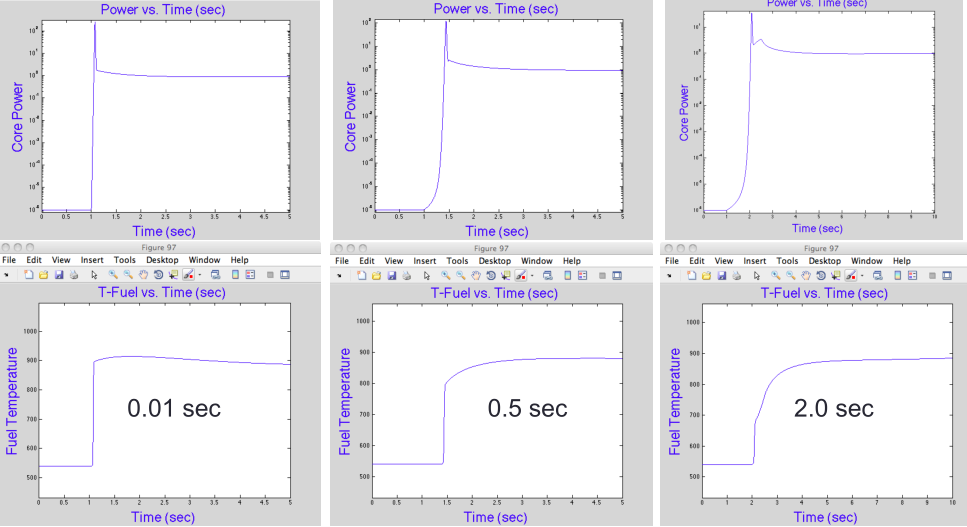
\includegraphics[width=6in]{images/pke/fn2.png}
    \caption{Fuel Temperature Independent Reactivity Insertion Rate} \label{fn2}
  \end{figure}

\item \$1.8 Insertion at Full Power: RIA at full power results in much smaller power increase because we are already at the point of sensible heat addition. Fuel temperature rise is similar to that of RIA from low power. 
  \begin{figure}[ht] 
    \centering
    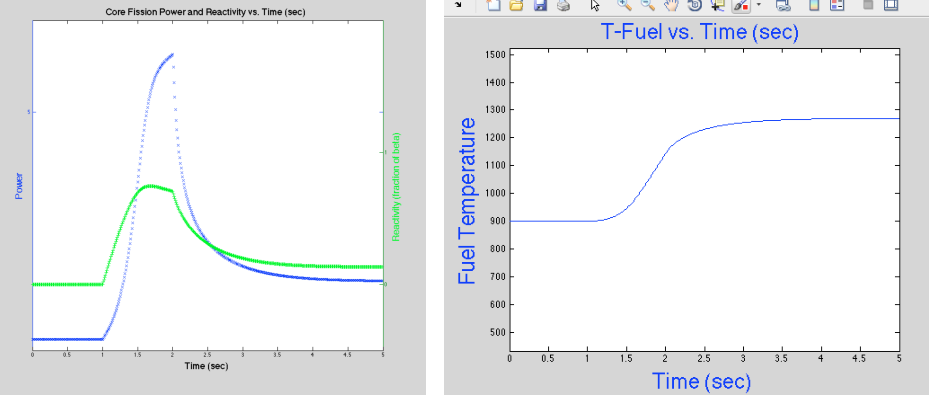
\includegraphics[width=4in]{images/pke/fn3.png}
    \caption{\$1.8 Insertion at Full Power using IK with Feedback}
  \end{figure}

\clearpage
\item As in Fig.~\ref{fn4}, about 3\% of the energy deposited into the coolant (about $2.5 \times 2$ MeV $=$5 MeV worth of neutrons from 200 MeV just from neutron slowing down that is deposited into the coolant), hence the coolant temperature would change slightly as well. Net reactivity comes back to zero.
  \begin{figure}[ht] 
    \centering
    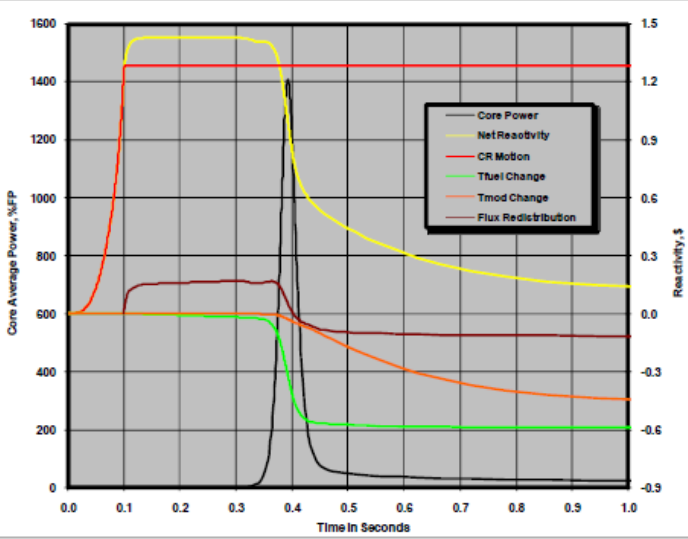
\includegraphics[width=4in]{images/pke/fn4.png}
    \caption{PWR Reactivity Insertion Accident} \label{fn4}
  \end{figure}

\item RIA Safety Analysis: Rod Ejection at HZP. If we have a 1.5\$ RIA without feedback, the power increases very rapidly with an asymptotic period. With Doppler feedback, the feedback is pronound when reactivity is above 1 dollar. A second peak is the characteristic of longer rod change. 
\end{enumerate}

\clearpage
\topic{PKEs with Simple Feedback}
We start with two first order ODEs, one for $T_{fuel}$, one for $T_{coolant}$, 
\begin{align}
\ddt T_{fuel} (t) &= a P(t) - b [T_{fuel}(t) - T_{coolant}(t)] \\
\ddt T_{coolant} (t) &= c [T_{fuel}(t) - T_{coolant} (t) ] - d [T_{coolant} (t) - T_{inlet} (t) ] 
\end{align}
Re-write in matrix form, 
\begin{align}
\ddt \left[ \begin{array}{c} T_{fuel}(t) \\ T_{coolant} (t) \end{array} \right]
+ \left[ \begin{array}{cc} b & -b \\ -c & c+d \end{array} \right] 
\left[ \begin{array}{c} T_{fuel} (t) \\ T_{coolant} (t) \end{array} \right] 
= 
\left[ \begin{array}{c} a P_{fuel}(t) \\ d T_{inlet}(t) \end{array} \right]
\end{align}
Using integrating factors to solve the above first order ODE system,  we get, 
\begin{align}
 \left[ \begin{array}{c} T_{fuel}^{n+1} \\ T_{coolant}^{n+1} \end{array} \right]
&= \exp \left\{ -  \left[ \begin{array}{cc} b & -b \\ -c & c+d \end{array} \right] \Delta_t^n \right\}
\left[ \begin{array}{c} T_{fuel}^n \\ T_{coolant}^n \end{array} \right] \\
&+ \exp \left\{ -  \left[ \begin{array}{cc} b & -b \\ -c & c+d \end{array} \right] \Delta_t^n \right\}
\left[ \begin{array}{cc} b & -b \\ -c & c+d \end{array} \right]^{-1}
\exp \left\{ \left[ \begin{array}{cc} b & -b \\ -c & c+d \end{array} \right] \Delta_t^n \right\}
\left[ \begin{array}{c} a P_{fuel}^{n+1} \\ d T_{inlet}^{n+1} \end{array} \right]
\end{align}
Some common initilization conditions could be, at full power flow rate is 30w/g, $C_p = 300$J /kg s, $\alpha = -3$ pcm/K, $V_{coolant} = 2 \m/\s, T_{inlet}^0 = 540 \K, T_{coolant}^0 = 560 \K, T_{fuel}^0 = 1000 \K$. 

Example: Ramp reactivity inertion of $\pm 0.5\beta$ with feedback. 
\begin{figure}[ht]
  \centering
  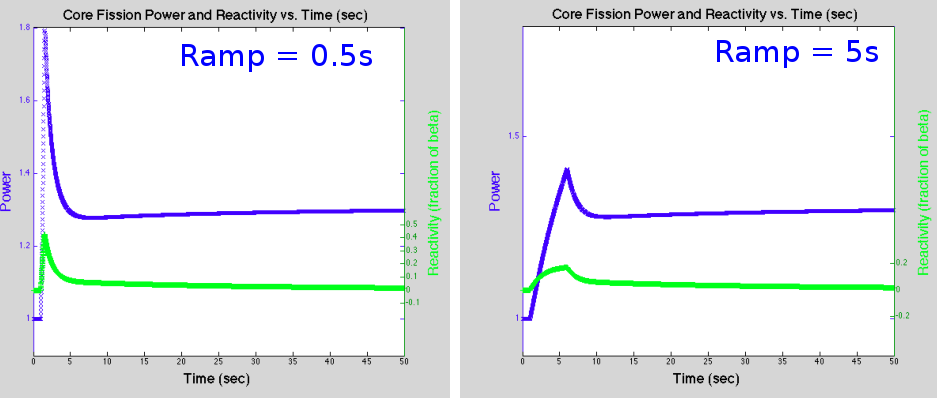
\includegraphics[width=4in]{images/pke/fn5.png}
  \caption{$0.5 \beta$ Reactivity Insertion with Feedback}
\end{figure}
\begin{figure}[ht]
  \centering
  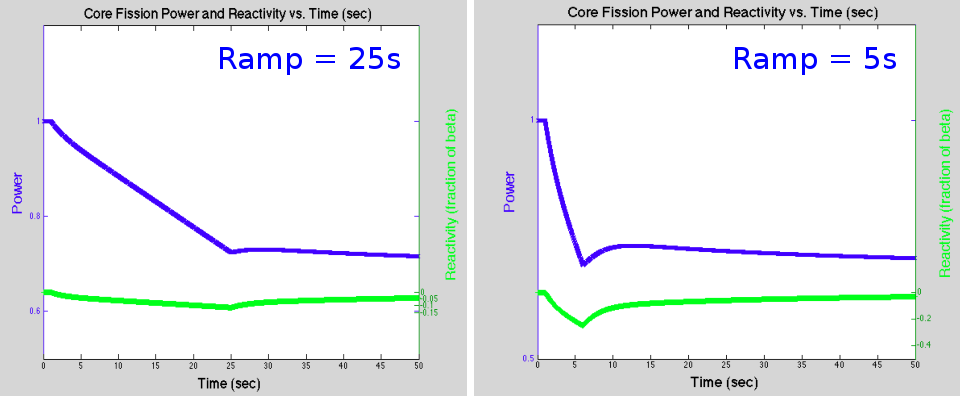
\includegraphics[width=4in]{images/pke/fn6.png}
  \caption{$-0.5 \beta$ Reactivity Insertion with Feedback}
\end{figure}
The slower ramping results in smaller reactivity change (hence smaller peak reactivity for reactivity insertion and larger power dip for negative reactivity insertion), thus smaller power change as well. That is, \textbf{The smaller rate of reactivity change is, the smaller the overshoot is.} But the final/asymptotic results are independent of rate of reactivity insertion, because system always finds stable state. 

Selective ramp insertion: 2 sec, power comes down quickly and recoveries, the radial heat gets high, close to an DNDF failure, makes sure to take into account the power rise. 

 

\topic{Summary}
\begin{enumerate}
\item PKEs assume you are solving for the core average properties; PKEs assume flux spatial shape is constant. Thus PKEs are not very precise for large spatial flux changes. 
\item Peak temperature are proportionally larger than core average properties;
\item If we relly want spatial dynamics, we need to do 3D spatial dynamics to get correct predictions to complicated problems. 
\end{enumerate}


\end{document}
